\documentclass[a4paper,12pt]{article} % тип документа

% report, book

%  Русский язык
\usepackage{multirow}
\usepackage{wrapfig}
\usepackage[T2A]{fontenc}			% кодировка
\usepackage[utf8]{inputenc}			% кодировка исходного текста
\usepackage[english,russian]{babel}	% локализация и переносы
\usepackage{booktabs}
\usepackage{indentfirst} %Красная строка
\usepackage[a4paper,top=1.3cm,bottom=2cm,left=1.5cm,right=1.5cm,marginparwidth=0.75cm]{geometry}
\usepackage[usenames]{color}
\usepackage{colortbl}

% Заметки
\usepackage{todonotes}

% Математика
\usepackage{amsmath,amsfonts,amssymb,amsthm,mathtools} 
\usepackage{graphicx, wrapfig, subcaption, setspace, booktabs}
\usepackage{hyperref}
\usepackage{caption} % подписи к рисункам в русской типографской традиции
\DeclareCaptionFormat{GOSTtable}{#2#1\\#3}
\DeclareCaptionLabelSeparator{fill}{\hfill}
\DeclareCaptionLabelFormat{fullparents}{\bothIfFirst{#1}{~}#2}
%\captionsetup[table]{
 %    format=GOSTtable,
  %   font={footnotesize},
   %  labelformat=fullparents,
    % labelsep=fill,
     %labelfont=it,
%     textfont=bf,
 %    justification=centering,
  %   singlelinecheck=false
   %  }


\begin{document}

\begin{titlepage}
\begin{center}
    {\large МОСКОВСКИЙ ФИЗИКО-ТЕХНИЧЕСКИЙ ИНСТИТУТ (НАЦИОНАЛЬНЫЙ ИССЛЕДОВАТЕЛЬСКИЙ УНИВЕРСИТЕТ)}
\end{center}
\begin{center}
    {\largeФизтех-школа биологической и медицинской физики}
\end{center}


    \vspace{3.5cm}

\begin{center}
    
\includegraphics[width=0.35\linewidth]{hv_full.png}
\end{center}
\vspace{0.1cm}
{\huge
\begin{center}
    {\bf Вопрос по выбору для ГКЭ по общей физике}\\
    Определение размера золотых наночастиц с помощью метода ДРС
\end{center}
}
\vspace{2cm}
\begin{flushright}
{\LARGE Волкова Анна \\
Хомутов Андрей \\ 
\vspace{0.2cm}
Б06-903}
\end{flushright}
\vspace{2.5cm}
\begin{center}
    Долгопрудный 2022
\end{center}
\end{titlepage}

\section{Теоретическое введение}
\subsection{Динамическое светорассеяние}
Процесс рассеяния света состоит в заимствовании молекулой или частицей некоторой доли энергии у распространяющейся в среде электромагнитной волны и излучении этой энергии в окружающее пространство. В результате могут происходить изменения характеристик потока излучения: пространственного распределения интенсивности, частотного спектра, поляризации.

Процесс рассеяния можно представить следующей схемой:
\begin{center}
    \textbf{Рассеяние = возбуждение + переизлучение}. 
\end{center}
При распространении в среде интенсивность падающего света ослабляется с расстоянием (закон Бугера-Ламберта-Бера): 
\begin{equation}
    I = I_0e^{-Sx}, 
\end{equation}
где $S$ – коэффициент экстинкции среды, $x$ – толщина слоя вещества.

Под возбуждением понимаются процессы поляризации частицы в результате ее взаимодействия с электромагнитным полем, т.е. наведение в частице переменного дипольного момента. 

Рассеяние происходит на оптических неоднородностях среды, возникающих при изменении показателя преломления. Оптическая неоднородность среды может быть связана с присутствием в ней диспергированных частиц. Однако даже в средах, которые можно считать однородными, имеют место флуктуации плотности. В результате среда становится оптически неоднородной, и на этих неоднородностях рассеивается свет.

Возникновение и исчезновение флуктуаций разных величин происходит за различное время. Так флуктуация плотности представляет собой упругую волну, которая распространяется в жидкости со скоростью звука, а ее затухание обусловлено вязкостью среды. 

\subsection{Динамическое рассеяние}
Методы динамического светорассеяния позволяют определить время жизни флуктуации. В данной работе использовался метод фотонной корреляционной спектроскопии. С его помощью изучается корреляция (во времени) количества фотонов, рассеянных образцом в заданном направлении. В качестве источника излучения используется лазер. Электромагнитные волны, рассеянные соседними частицами, интерферируют друг с другом. Возникающие при этом временные флуктуации интенсивности рассеянного света формируют на фотодетекторе сигнал $I(t)$, характерные времена изменения которого обусловлены броуновским движением рассеивающих частиц.

Эти флуктуирующие сигналы анализируются устройством, называемым коррелятором, который строит автокорреляционную функцию сигнала $I(t)$. Автокорреляционная функция показывает корреляцию значений интенсивности рассеянного света измеренных через промежуток времени $\tau$:

\begin{equation}
g(\tau)=\langle I(t) \cdot I(t+\tau)\rangle.
\end{equation}

Усреднение проводится по различным начальным моментам времени $t$:

\begin{equation}
\langle I(t) \cdot I(t+\tau)\rangle=\lim _{\Delta t \rightarrow \infty} \frac{1}{\Delta t} \int_{0}^{\Delta t} I(t) \cdot I(t+\tau) d t.
\end{equation}

Таким образом, автокорреляционная функция (АКФ) сигнала представляет собой интеграл от произведения двух копий сигнала, сдвинутых относительно друг друга на время $τ$.

\begin{center}
\begin{figure}[h!]
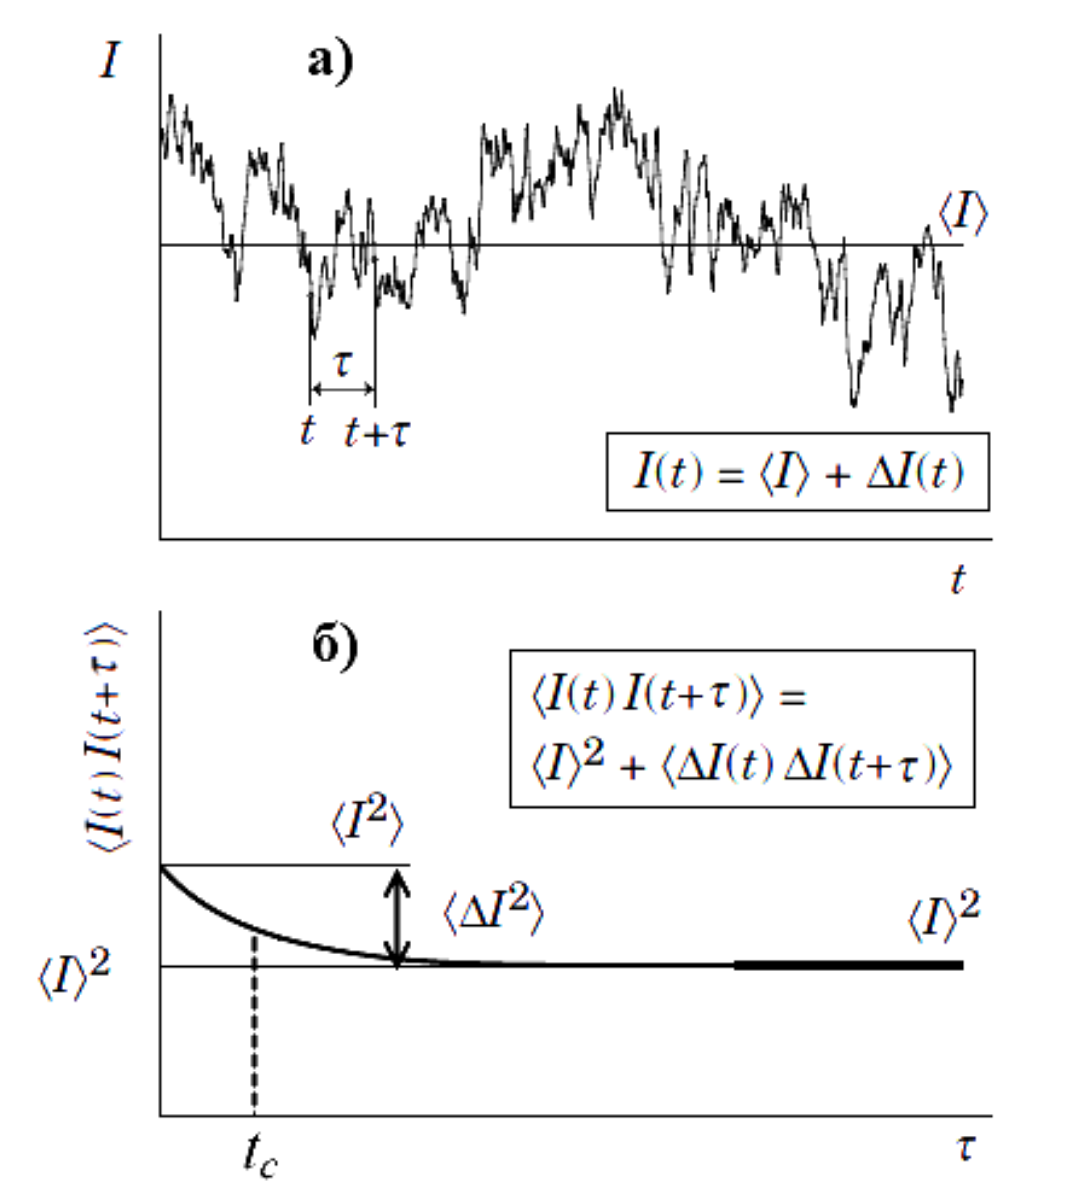
\includegraphics[width=0.6\textwidth]{afk.png}
\caption{Изменение интенсивности рассеянного света во времени (а) и соответствующая автокорреляционная функция (б) }
\end{figure}
\end{center}

На схеме (Рис. 2) показано, что при падении плоской электромагнитной волны с волновым вектором \boldsymbol{k} на рассеивающий объект происходит переизлучение световых волн по различным направлениям. При этом световой поток в первоначальном направлении ослабляется. Угол рассеяния $\theta$, под которым производится регистрация рассеянного излучения, определяет волновой вектор рассеяния для данного направления наблюдения. Здесь \boldsymbol{k} – волновой вектор падающего света, $\boldsymbol{q}=\boldsymbol{k}-\boldsymbol{k}^{\prime}$ – волновой вектор рассеянния. При упругом рассеянии $|\mathrm{k}| \approx\left|\mathrm{k}^{\prime}\right|$ и модуль волнового вектора рассеяния  выражается через длину волны света в вакууме $\lambda_0$ и показатель преломления растворителя $n$:

\begin{equation}
q=|\boldsymbol{q}|=2|\boldsymbol{k}| \cdot \sin \frac{\theta}{2}=\frac{4 \pi n}{\lambda_{0}} \sin \frac{\theta}{2}.
\end{equation}

\begin{figure}[h!]
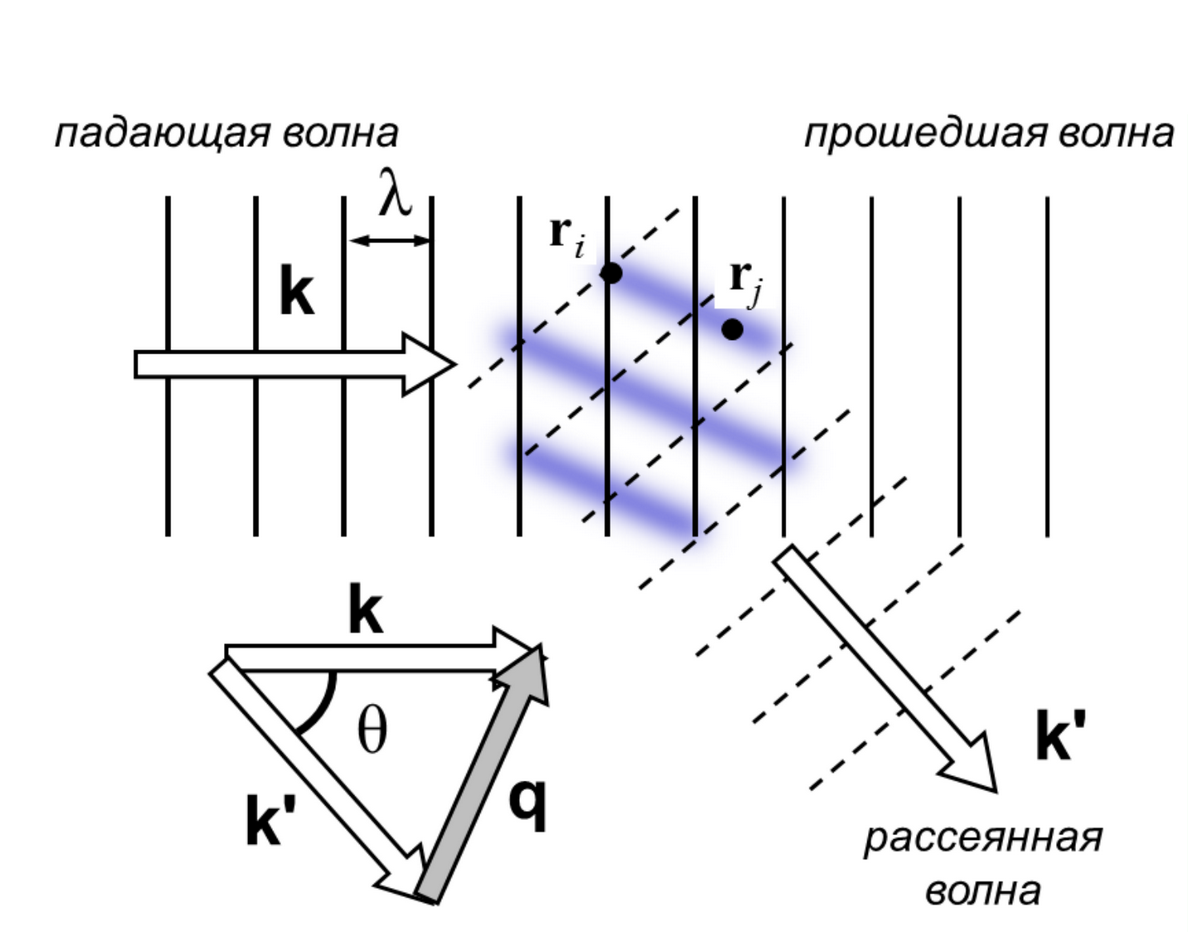
\includegraphics[width=0.8\textwidth]{shema.png}
\caption{Рассеяние на флуктуациях плотности}
\end{figure}

Вектор рассеяния \boldsymbol{q} задает фазовые сдвиги $\Delta \varphi_{i j}=\boldsymbol{q}\left(\boldsymbol{r}_{i}-\boldsymbol{r}_{j}\right)$ при сложении электромагнитных колебаний, приходящих на фотодетектор от различных элементарных диполей $i$ и $j$ внутри рассеивающего объема. Действительно,
$$
\Delta \varphi_{i j}=\varphi_{i} - \varphi_{i} = \boldsymbol{k'}\boldsymbol{r}_i - \boldsymbol{k'}\boldsymbol{r}_j - \boldsymbol{k}(\boldsymbol{r}_j-\boldsymbol{r}_i) = (\boldsymbol{k} - \boldsymbol{k'})(\boldsymbol{r}_i - \boldsymbol{r}_j).
$$
Результат интерференции переизлученных волн зависит от направления и величины вектора \boldsymbol{q}. Поэтому интенсивность рассеянного излучения может зависеть от угла $\theta$. 

Флуктуации диэлектрической проницаемости могут быть представлены в виде пространственного фурье-разложения – множества синусоидальных компонент. При заданном угле регистрации θ рассеяние света на флуктуациях можно рассматривать как дифракцию на одной пространственной фурье-компоненте флуктуации, волновой вектор которой равен вектору рассеяния \boldsymbol{q}. Рассеивающие центры $i$ и $j$ расположены так, что фазовые сдвиги рассеянных ими волн  кратны $2\pi$, т.е. обеспечивают интерференцию с усилением, то есть выполняет условие Брэгга. 

Электрическое поле световой волны, рассеянной на флуктуациях показателя преломления среды в направлении вектора $\boldsymbol{k}^{\prime}$, можно представить в виде:

\begin{equation}
E(t)=\delta E(t) \cdot e^{-i \omega_{0} t},
\end{equation}

где медленно меняющаяся со временем амплитуда поля $\delta E(t)$
пропорциональна флуктуации концентрации рассеивающих частиц:

\begin{equation}
\delta C_{\mathrm{q}}(\boldsymbol{r}, t)=\delta A_{\mathrm{q}}(t) \cdot \sin (\boldsymbol{q} \boldsymbol{r}),
\end{equation}

\begin{equation}
\delta E(t)=A \cdot \delta C_{\mathbf{q}}(\mathrm{r}, t).
\end{equation}

Здесь подразумевается, что флуктуации представлены в виде пространственного фурье-разложения.

В соответствии с гипотезой Онзагера, релаксация микроскопических флуктуаций к равновесному состояниию может быть описана уравнением диффузии:

\begin{equation}
\frac{\partial C}{\partial t}=D \nabla C,
\end{equation}

решая это уравнение, можно получить:

\begin{equation}
\delta C_{\mathbf{q}}(\boldsymbol{r}, \tau)=\delta C_{\mathbf{q}}(\boldsymbol{r}, 0) \cdot \exp \left(-D q^{2} \tau\right)=\delta C_{\mathbf{q}}(\boldsymbol{r}, 0) \cdot \exp \left(-\frac{\tau}{t_{c}}\right),
\end{equation}

где 

\begin{equation}
\frac{1}{t_{c}}=D q^{2}
\end{equation}

есть обратное время жизни такой флуктуации.

Из формулы Стокса-Эйнштейна,

\begin{equation}
D=\frac{k T}{6 \pi \eta R},
\end{equation}

можно определить размеры рассеивающих наночастиц в растворе. 

Автокорреляционная функция интенсивности рассеянного света имеет вид:

\begin{equation}
\langle I(t) I(t+\tau)\rangle=A \exp \left(-\frac{2 \tau}{t_{c}}\right)+B.
\end{equation}

\subsection{Индикатрисса рассеяния}

Индикатриса рассеяния – кривая, графически отображающая зависимость интенсивности рассеянного света от угла рассеяния. В общем случае индикатриса рассеяния не выражается явной функцией и описывается таблично либо в виде диаграмм в полярных или сферических координатах. Примеры индикатрисс для частиц разных размеров:

\begin{center}
\begin{figure}[h]
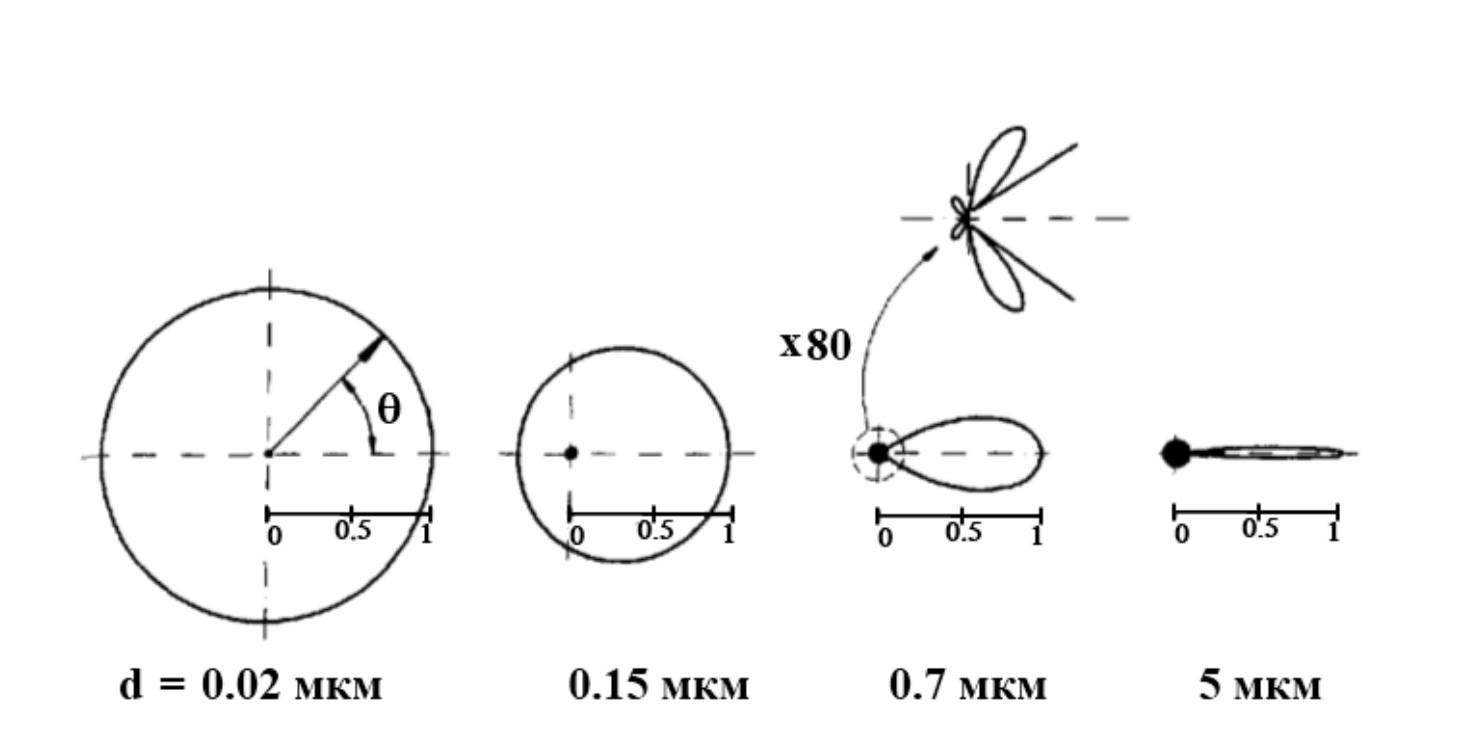
\includegraphics[width=1\textwidth]{Rj6DFQ7JDjk.jpg}
\caption{Типичный вид индикатрис рассеяния для частиц разного размера. Длина
волны падающего света в данном примере – 633 нм}
\end{figure}
\end{center}
Вид угловой зависимости рассеяния определяется размерами и формой рассеивающих частиц. Для рассеяния вертикально поляризованного излучени малыми частицами, размер которых много меньше длины волны излучения ($\lambda$/15), интенсивность рассеянного света не зависит от угла рассеяния при регистрации интенсивности. С увеличением размеров частицы интенсивность рассеянного света существенно возрастает, и в то же время изменяется угловое распределение рассеянного света: усиливается рассеяние вперед.
\clearpage


\section{Практическая часть}

Для эксперимента были использованы растворы наночастиц золота разных размеров. Подробнее о синтезе можно прочитать в разделе "Дополнения". Названия растворов по размеру частиц соответственно: S, M1, M2, M3, L.

\begin{figure}[h!]
    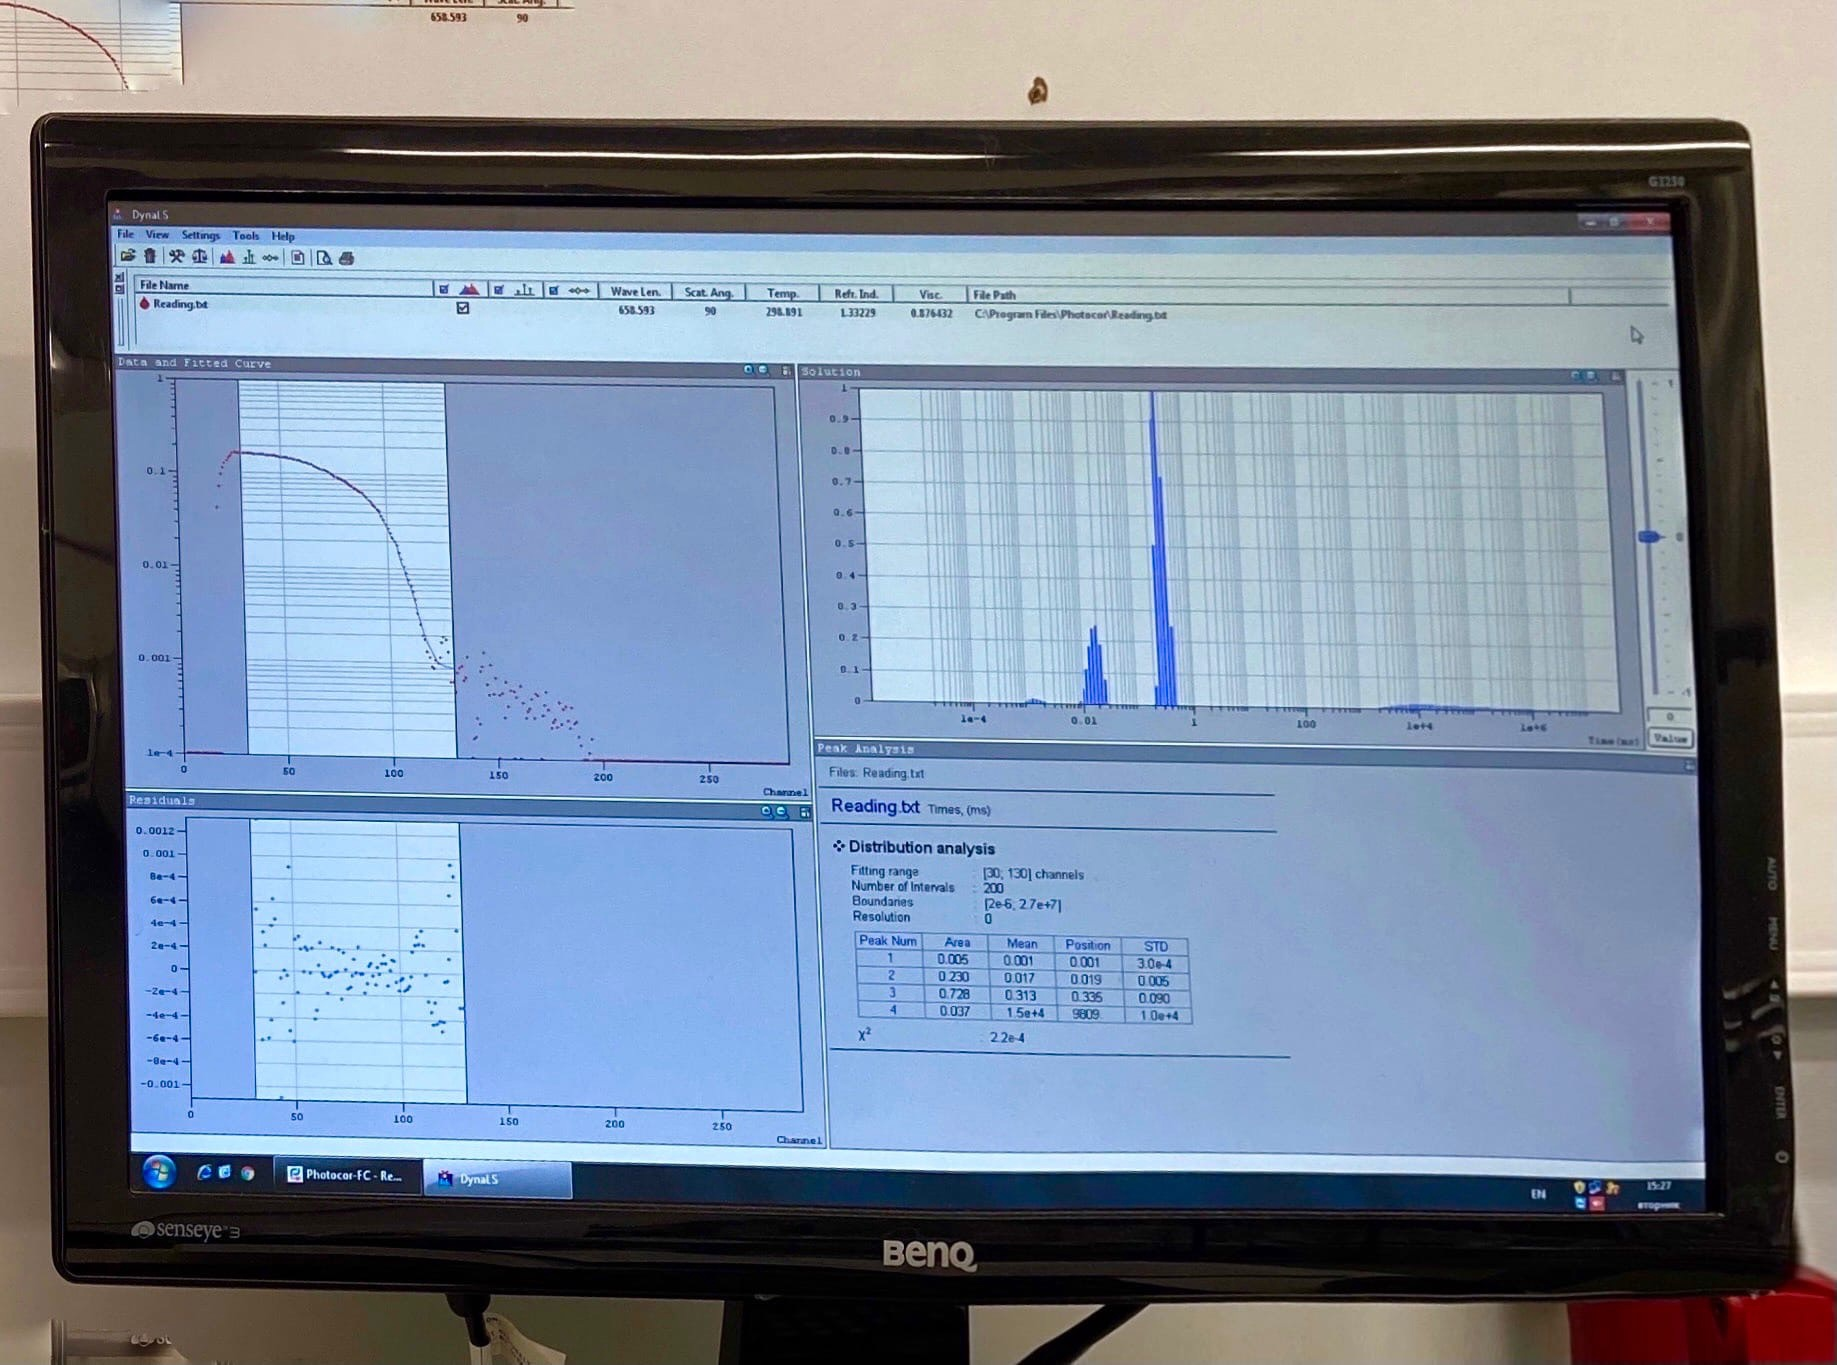
\includegraphics[width=1\textwidth]{222163047_457267330.jpg}
    \caption{Пример выводы программы}
\end{figure}

При помощи  спектрометра Photocor Complex были сняты АФК для различных углов и частиц. Оказалось, что у частиц наблюдается 2 характерестических времени. Одно по порядку величины составляло 0.1 - 1 мс, другое - значительно меньше, около 0.01 мс, причем оно не зависит от угла снятия. Последовало логичное предположение, что меньшее время отвечает вращательному движению частиц. С помощью модели Дебая-Стокса-Эйнштейна можно получить$^\text{[2]}$ характерное (дебаевское) корреляционное время $\tau_c = \frac{4\pi \eta a^3}{3kT}$, и с помощью него рассчитать размер наночастиц еще одним способом. Результаты представлены в таблице 1. Видно, что оба метода дали весьма близкие результаты.


\begin{table}[h]
\begin{center}
\caption{Расчетный размер наночастиц}
\begin{tabular}{|l|l|l|}
\hline
Обр. & $R_{\tau_1}$, нм & $R_{\tau_2}$, нм \\ \hline
S       & 20               & 17               \\ \hline
M1      & 25               & 24               \\ \hline
M2      & 26               & 24               \\ \hline
L       & 28               & 28               \\ \hline
\end{tabular}
\end{center}
\end{table}
%\clearpage

\begin{figure}[h!]
\begin{center}
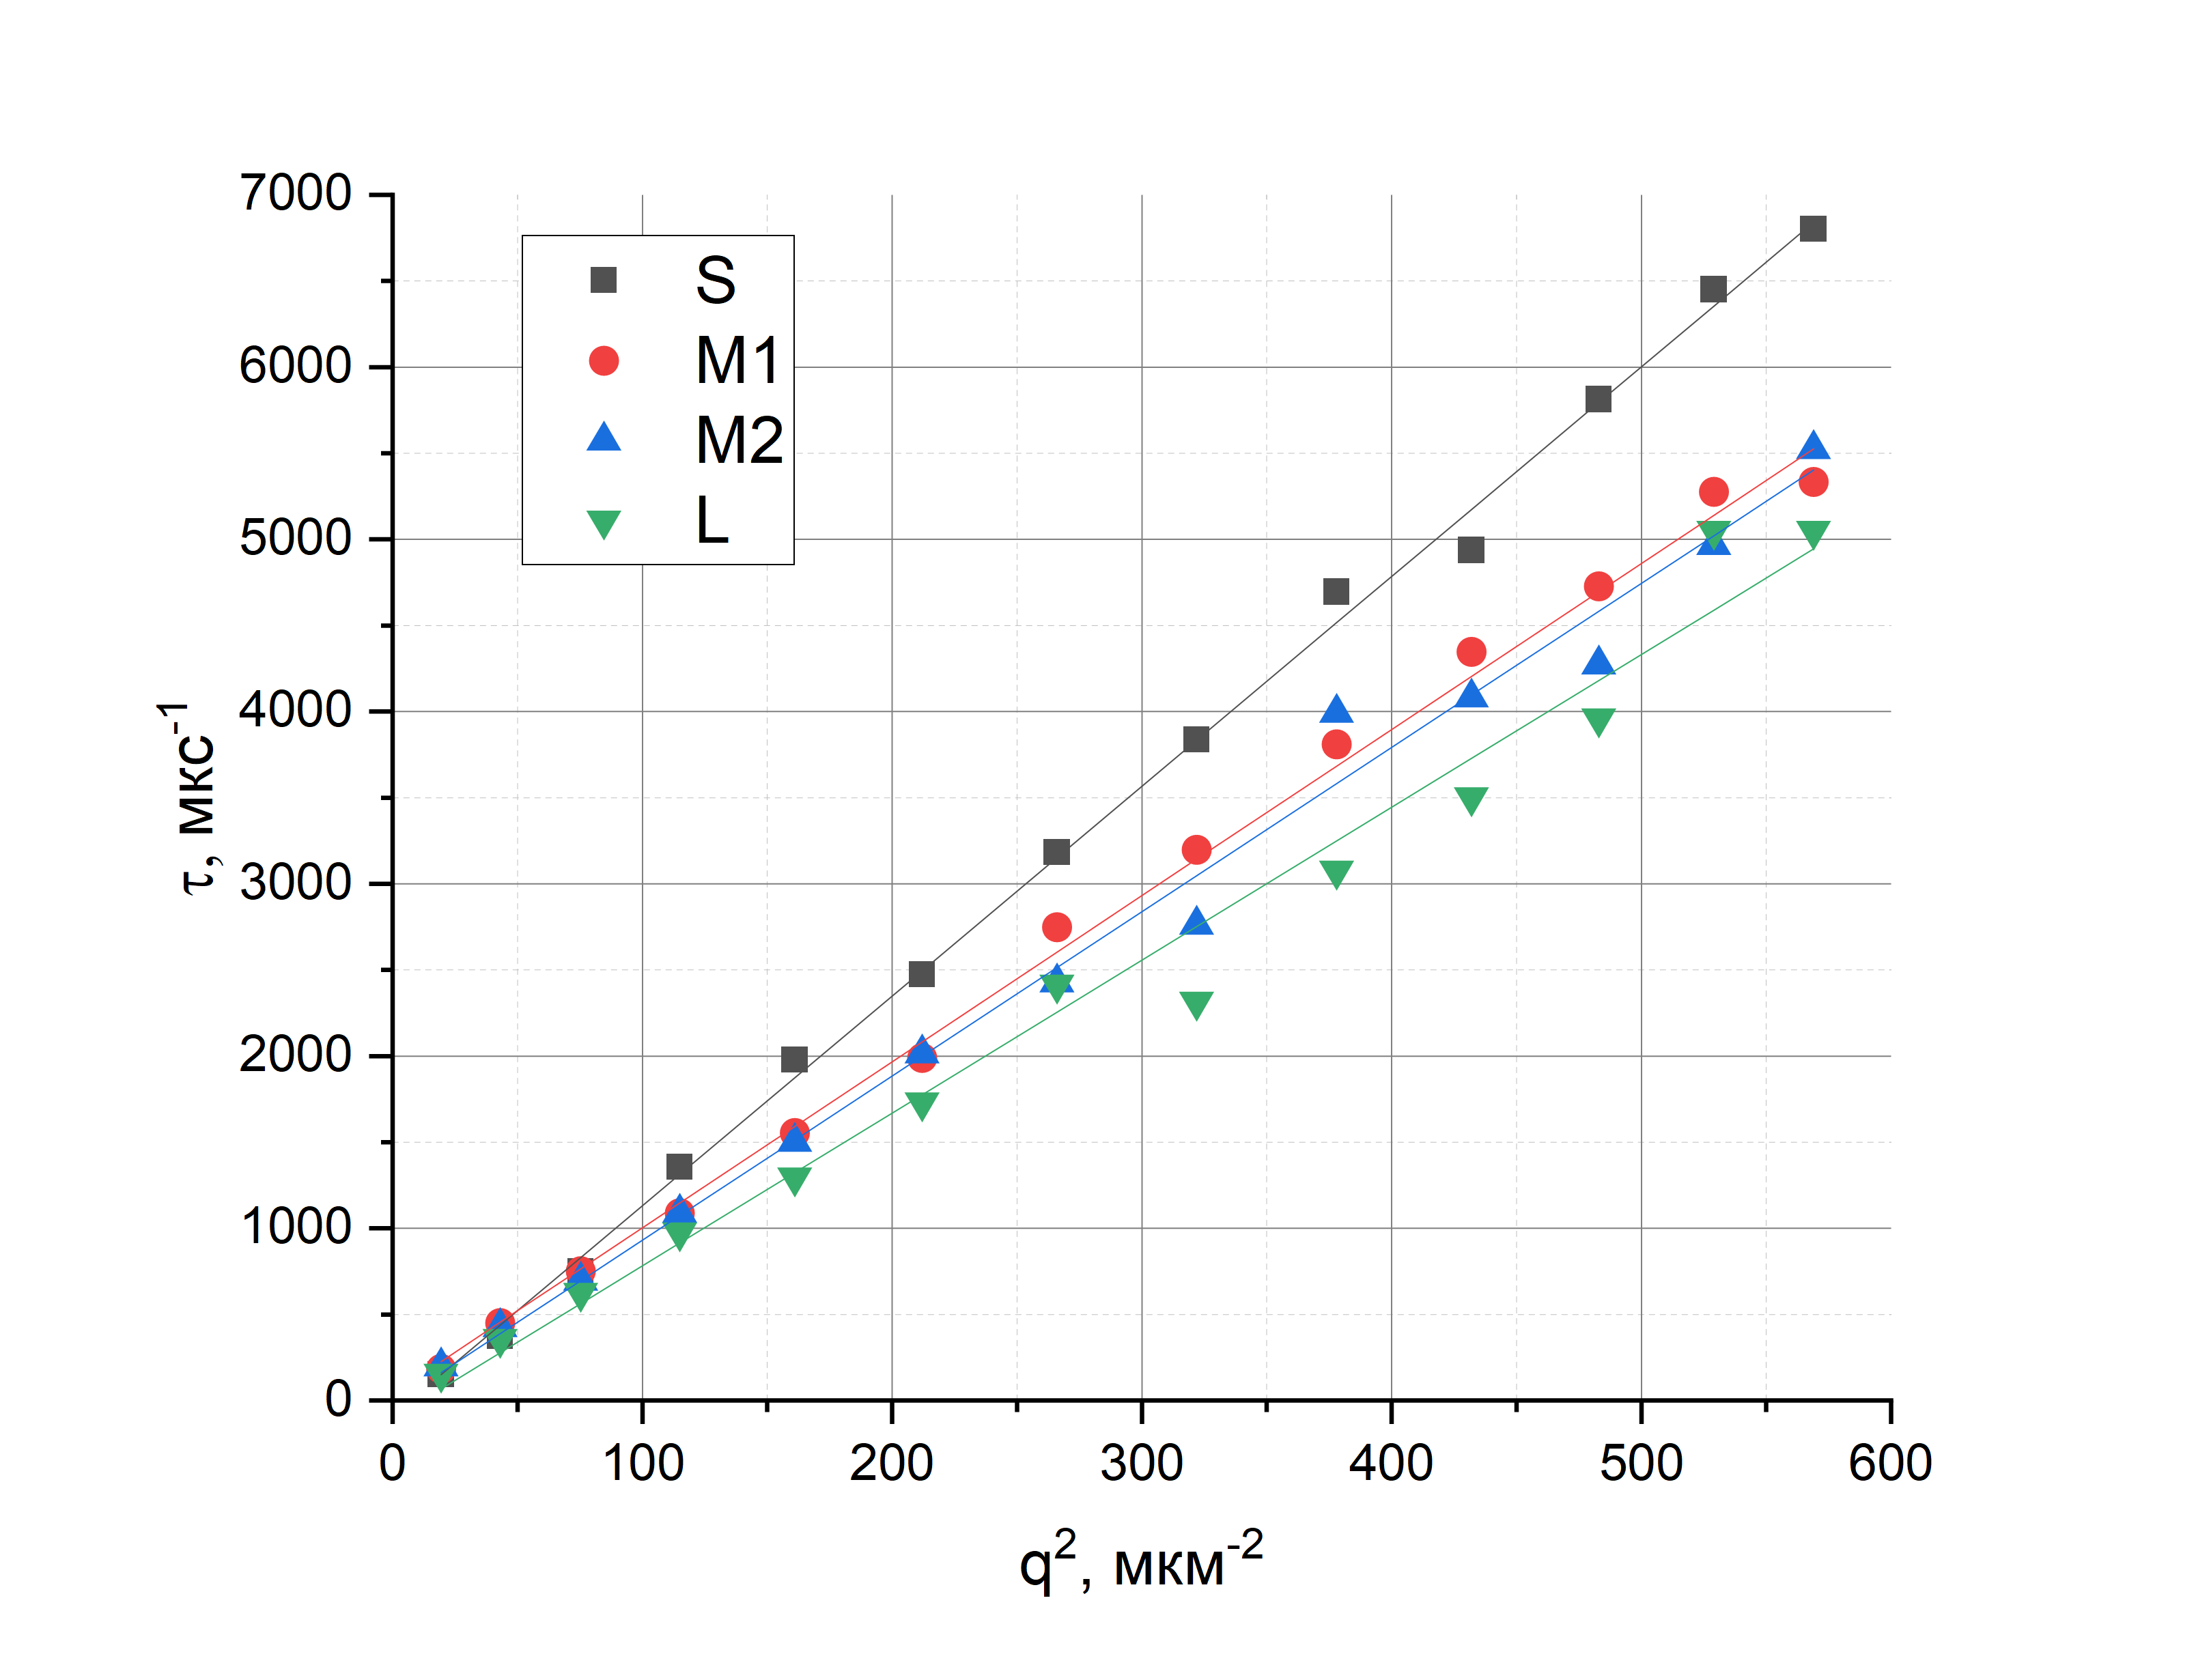
\includegraphics[width=0.8\textwidth]{D.png}
\caption{Графики для расчета коэффициента диффузии}
\end{center}
\end{figure}

Для образца L была снята зависимость интенсивности рассеянного излучения в зависимости от угла. Геометрические параметры установки позволили снять значения только в диапазоне от 20 до 140 градусов. По этим данным была построена диаграмма индикатриссы рассеяния.

\begin{figure}[h]
\begin{center}
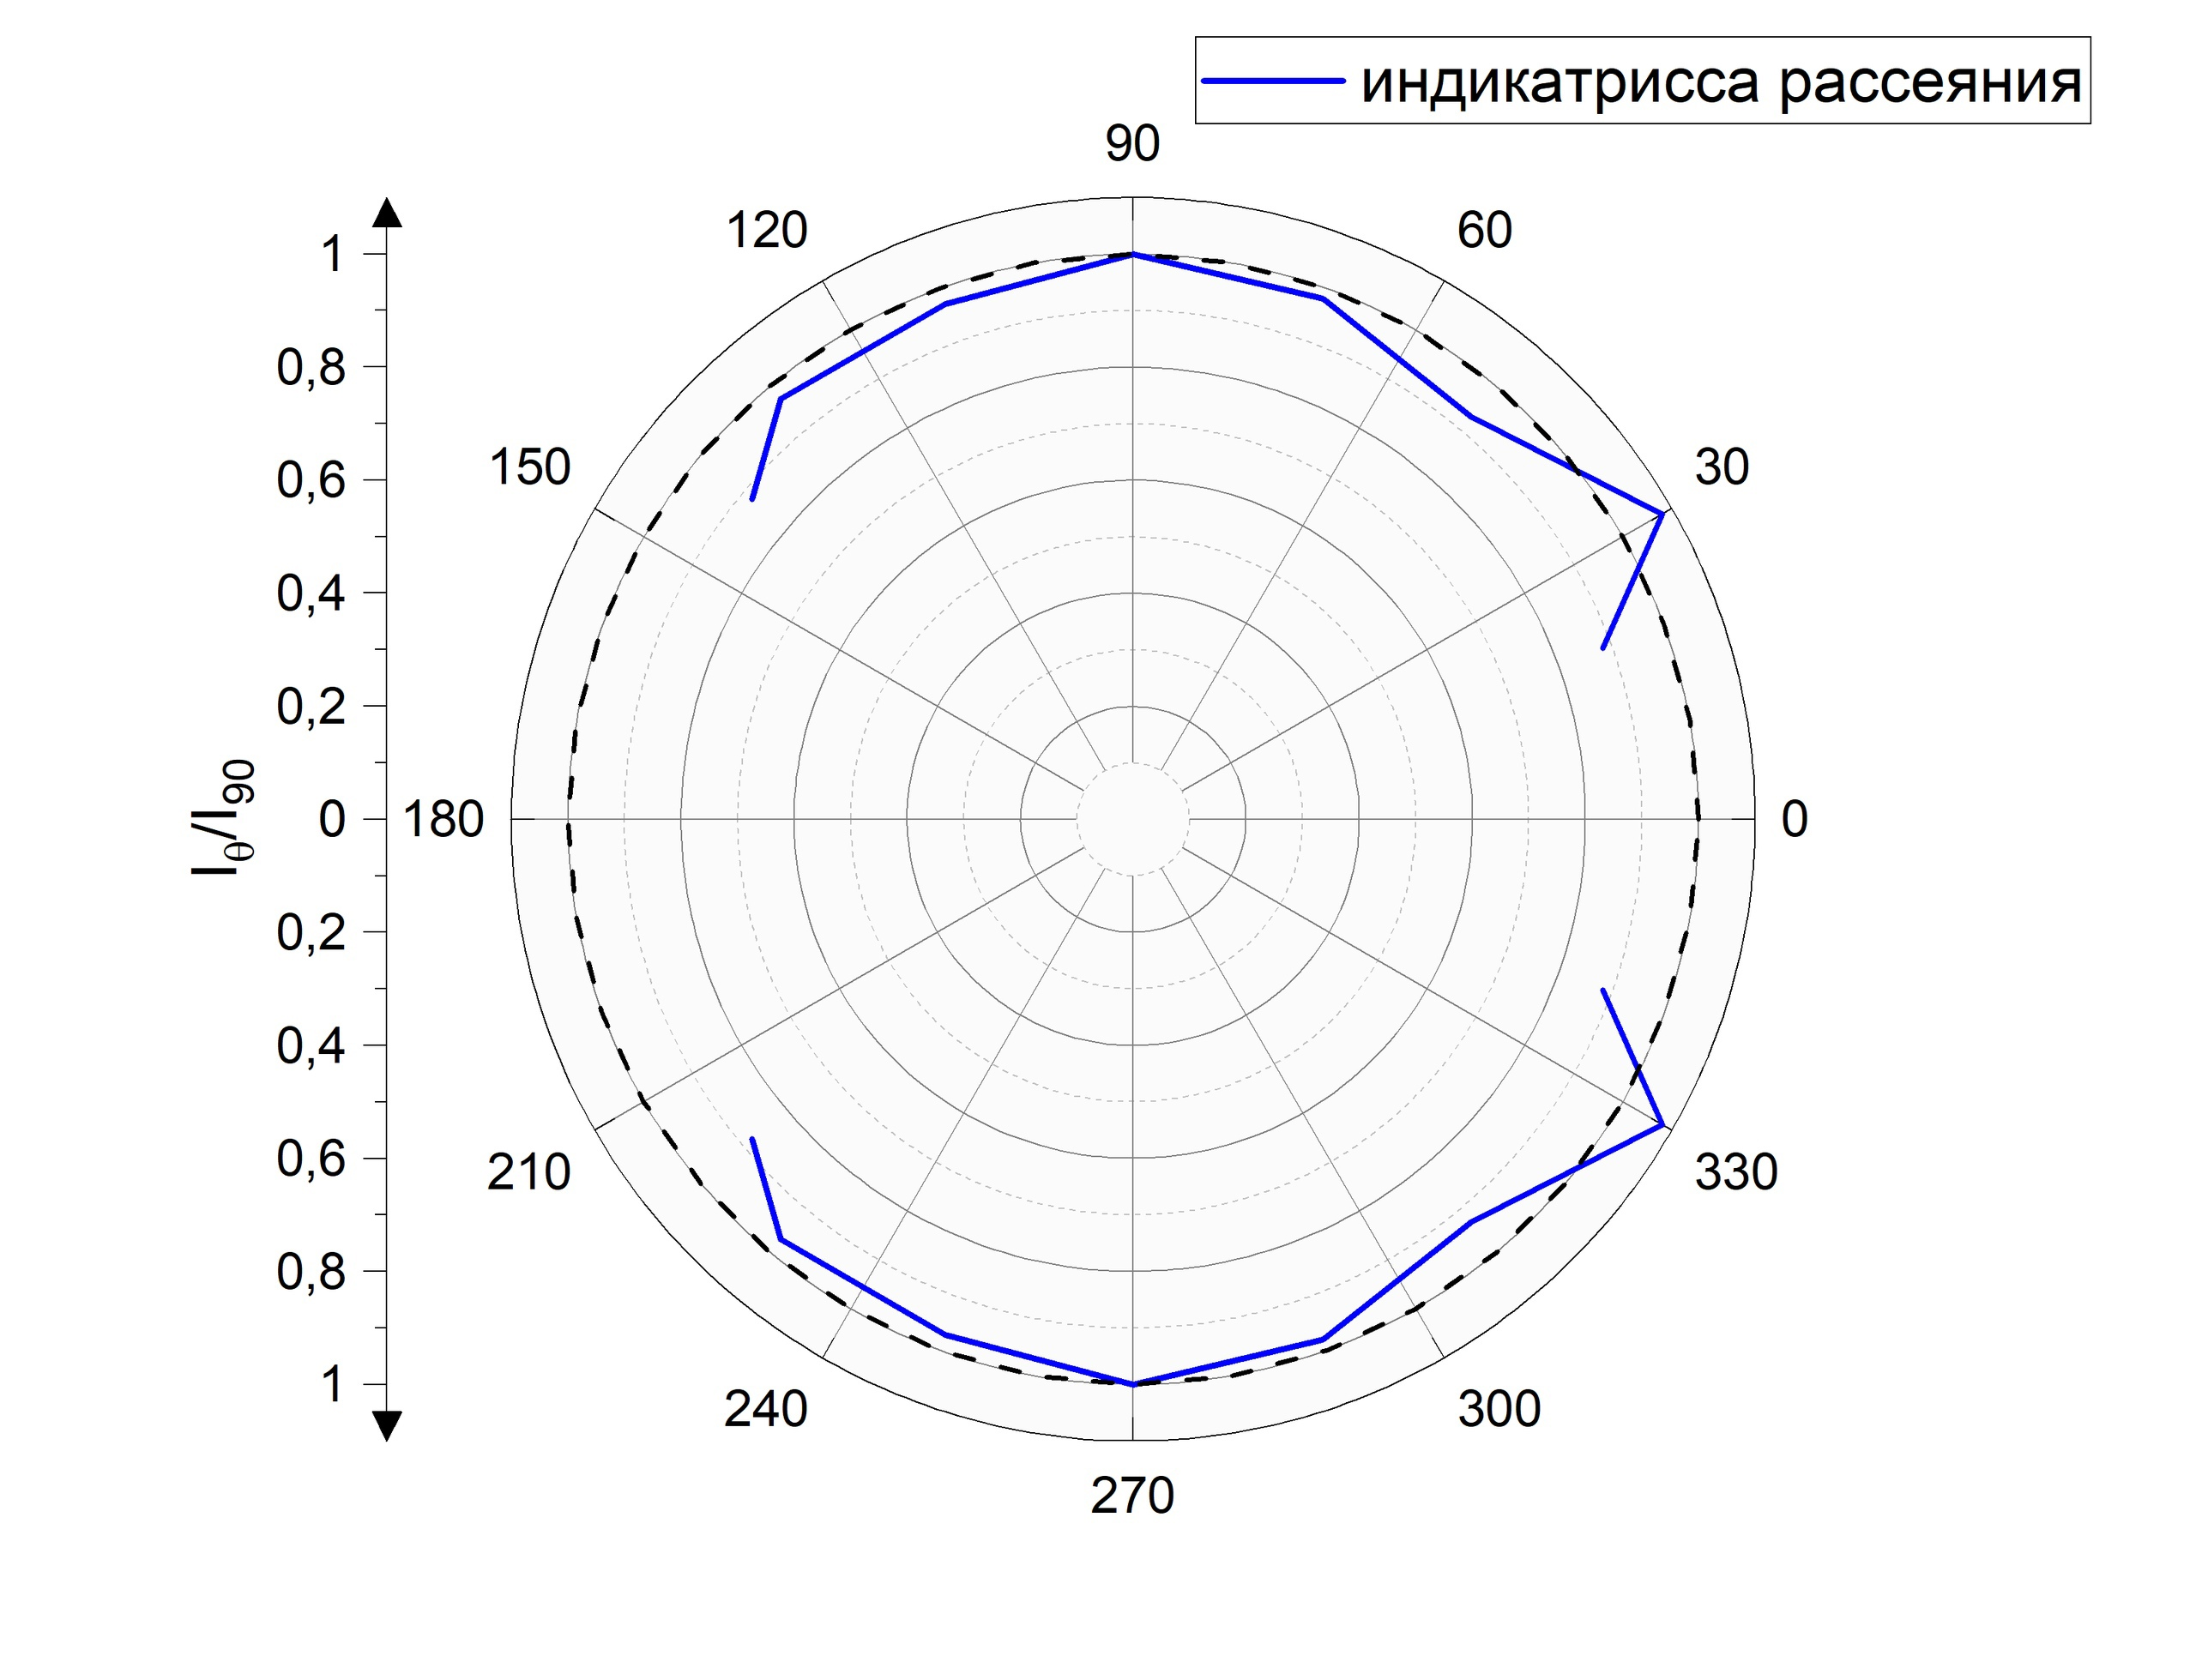
\includegraphics[width=0.8\textwidth]{x11jeDUvqWk.jpg}
\caption{Индикатрисса рассеяния для наночастиц образца L} %% подпись к рисунку
\end{center}
\end{figure}

\begin{figure}[h]
\begin{center}
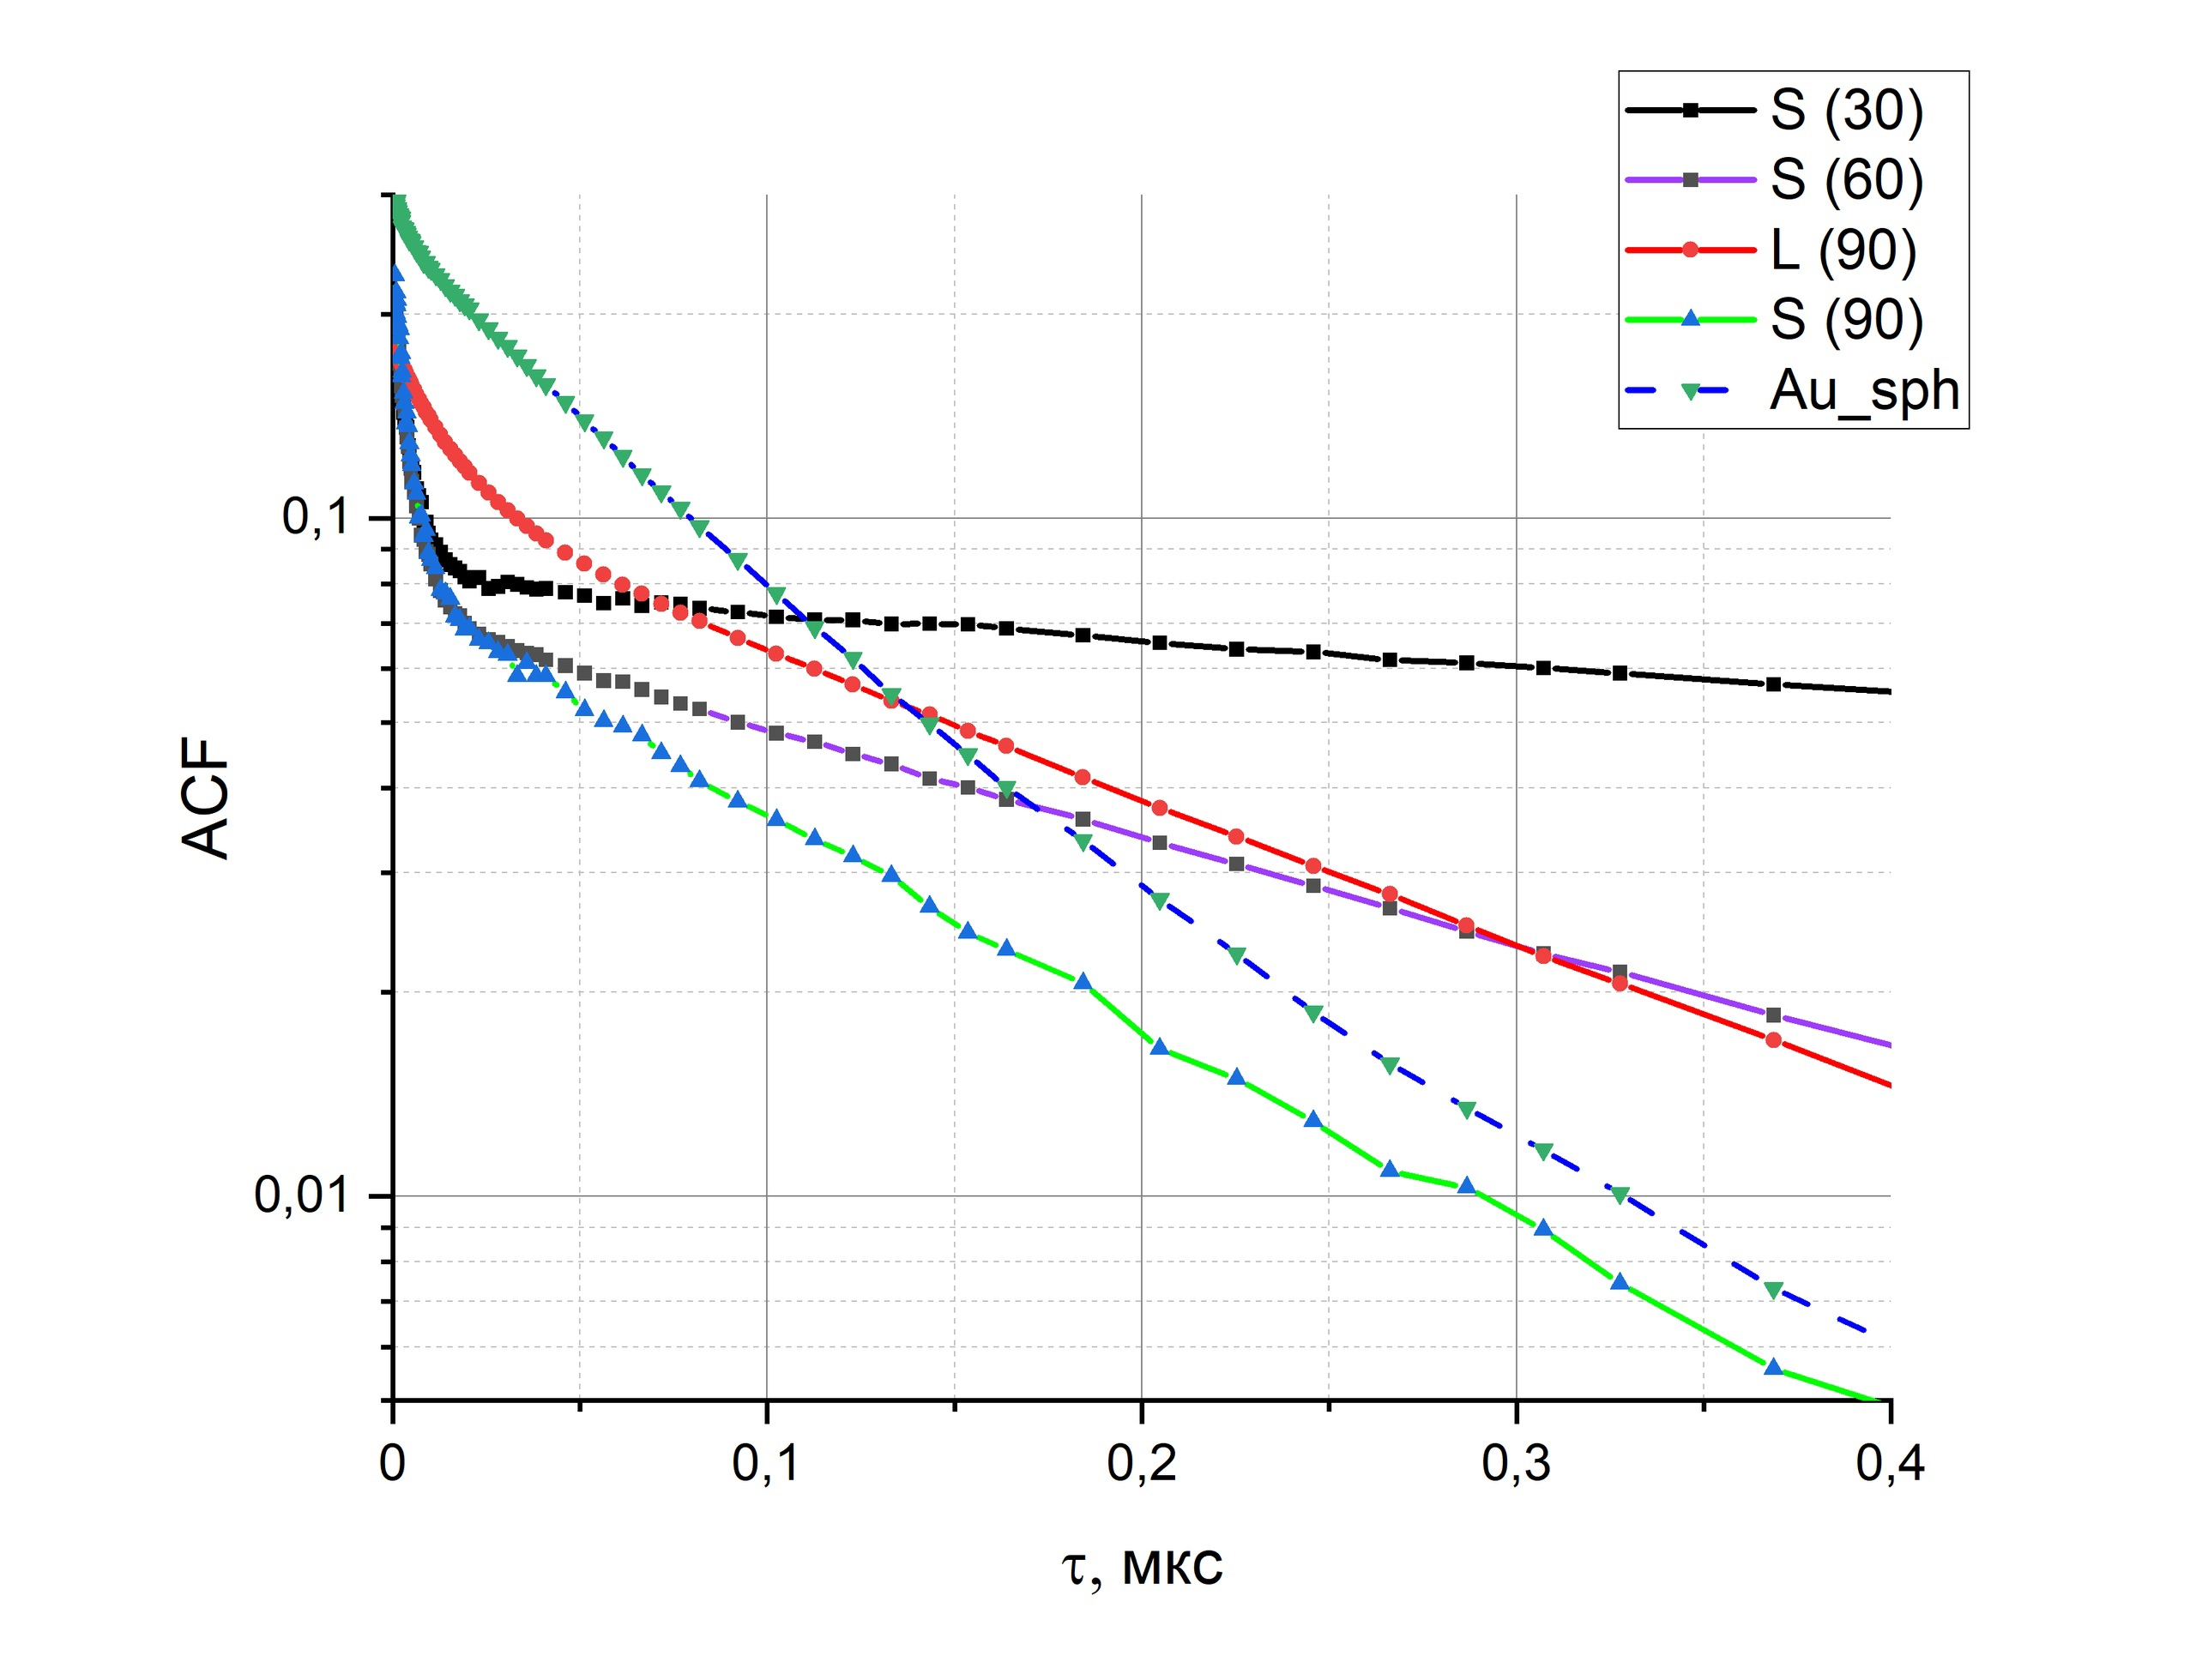
\includegraphics[width=0.8\textwidth]{_fBnuR-wyHo.jpg}
\caption{Графики зависимости ACF от времени}
\end{center}
\end{figure}



\clearpage

\section{Дополнения}

\subsection{Синтез наночастиц}
Был проведен синтез с вариацией по форме - от практически сферических до достаточно вытянутых цилиндров (сначала был синтезирован маточный раствор с маленькими зародышами, а потом различные его количества добавлялись к ростовому раствору, содержащему нитрат серебра и тетрахлороаурат водорода).


\begin{table}[h]
\begin{center}
\begin{tabular}{|l|l|l|}
\hline
Образец & V(AgNO3), мкл & V(маточного раствора), мкл \\ \hline
S       & 250           & 50                         \\ \hline
M1      & 50            & 12                         \\ \hline
M2      & 150           & 12                         \\ \hline
M3      & 250           & 12                         \\ \hline
L       & 250           & 1.5                        \\ \hline
\end{tabular}
\end{center}
\end{table}

\begin{figure}[h!]
    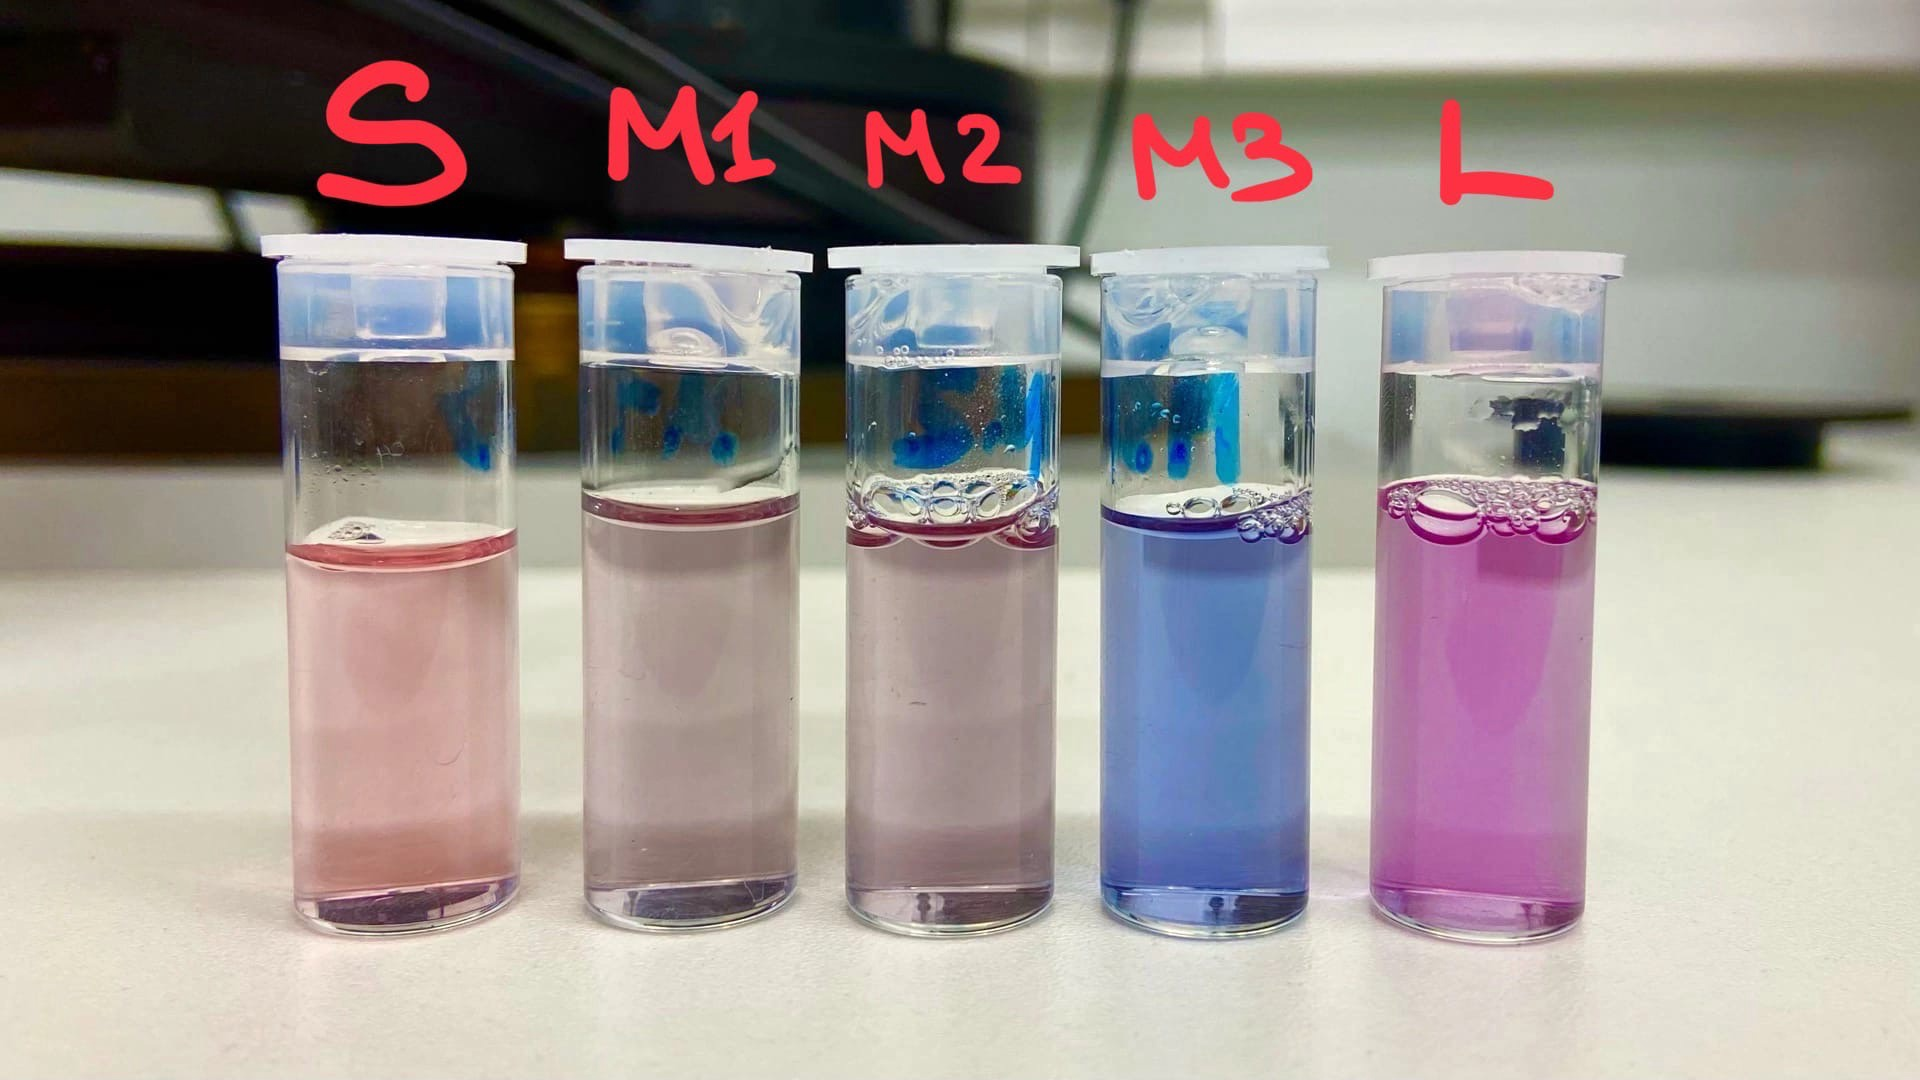
\includegraphics[width=0.9\textwidth]{7hGiKI_CvME.jpg}
    \caption{Наночастицы золота разных размеров}
\end{figure}

\section{Используемая литература литература}
\begin{enumerate}
    \item Методы статического и динамического рассеяния света для исследования наночастиц и макромолекул в растворах / К. В. Бочаров, Н. И. Марукович, А. Ю. Куксин - 2016
    \item Магнитный резонанс и его применение в химии / Керрингтон А., Мак-Лечлан Э. - 1970

\end{enumerate}


\end{document}
